\documentclass[12pt, letterpaper]{article} 

\usepackage{amsmath, amssymb, amsthm, enumerate, graphicx}

\title{MATH  HW }
\author{Dani Nguyen}
\date{Winter 2025}

\begin{document}
\maketitle
\graphicspath{ {./} }

\noindent \textbf{Question 1}\
\begin{enumerate}[a.]
    \item 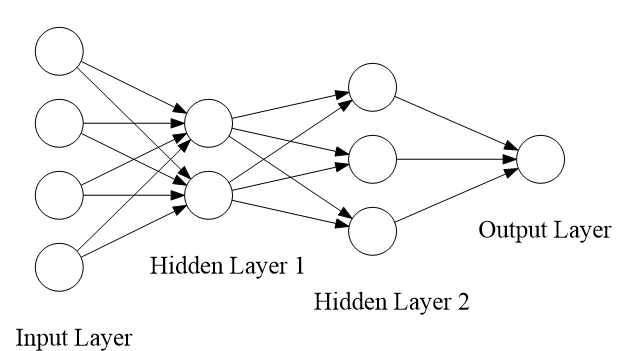
\includegraphics[scale=0.8]{neural_network.png}
\end{enumerate}

\noindent \textbf{Question 2} 
\begin{enumerate}[a.]
    \item \ 
    \item \ 
    \item The constraints are from the convolution filters being $5\times 5$, meaning 
    in the input image, only 25 pixels will impact one pixel on the convolved image, 
    
    A lot of the parameters are also repeated because the 

\end{enumerate}
\noindent \textbf{Question 3} \\

\end{document}